
\section{Events and Probability}
$P(A)=\frac{k}{n}=\frac{\text{number of good outcomes}}{\text{total number of possible outcomes}}=\frac{|A|}{|\Omega|}$\\

\vspace{5mm}
 
	\begin{minipage}{8cm}
	\subsection{Probability \skript{16}}
		\begin{tabular}{ll}
			Codomain (Wertebereich):
			& ${0}\le{P(A)}\le{1}$\\ \\
			Certain (Sicheres) event:
			& $P(\Omega)=1$\\ \\
			Impossible event:
			& $P(\emptyset)=0$\\
			Subset (Untermenge) $A\subseteq B$: & $P(A)\leq P(B)$
		\end{tabular}
	\end{minipage}
		\begin{minipage}{11.2cm}
		\subsubsection{Calculation rules}
			\begin{tabular}{ll}
				Complementary event: &$P(\bar{A})=P({\Omega}\setminus{A})=1-P(A)$\\ \\
				Difference: &$P({A}\setminus{B})=P(A)-P({A}\cap{B})$\\ \\
				OR: &$P({A}\cup{B})=P(A)+P(B)-P({A}\cap{B})$\\
				AND (independent): & $P(A\cap B)=P(A)P(B)$
				
			\end{tabular}
		\end{minipage}
		\newline
		
\vspace{2mm}
\hrule

\vspace{3mm}


	\subsection{Independent events \skript{22}}
		\begin{minipage}{12cm}
			$A$ and $B$ are independent if:\\
			
			$P(A \mid B)=P(A)$ and $P(B \mid A)=P(B)$ is true.\\
			
			Then: \hspace*{8mm} $P(A\cap B)=P(A)P(B)$\\
		\end{minipage}
		\begin{minipage}{4cm}
			$ \cap \equiv AND $ \\
			$ \cup \equiv OR $\newline
		\end {minipage}\\
    	Die Tatsache, dass A eingetreten ist, hat keinen Einfluss auf die 
		Wahrscheinlichkeit von B.\\ 

		\vspace{2mm}
		\hrule
		\vspace{3mm}
		
	\subsection{Conditional probability of A given B / Bedingte Wahrscheinlichkeit \skript{18}}
		Die Wahrscheinlichkeit für das Eintreten des Ereignisses $A$ unter der
		Bedingung, dass das Ereignis $B$ bereits eingetreten ist.
		\begin{center}
		$P(A\mid B)= \dfrac{P(A\cap B)}{P(B)}=\underbrace{\frac{P(A)\cdot
		P(B)}{P(B)}=P(A)}_{\text{nur wenn unabhängig}}$ 
		\end{center}

	\vspace{2mm}
	\hrule
	\vspace{3mm}

\subsection{Bayes rule (Wahrscheinlichkeitsumkehr) \skript{18}}
		\begin{tabular}{ll}
		  $P(B\mid A)=P(A\mid B) \cdot\dfrac{P(B)}{P(A)} = \dfrac{P(A|B) P(B)}{\sum\limits_{i=1}^n P(A|B_i) P(B_i)}$\vspace{1mm}
		\end{tabular}
		
	\vspace{2mm}
	\hrule
	\vspace{3mm}

\subsection{Law of total probability \skript{19}}
  \begin{minipage}{10cm}
	  \begin{tabular}{ll}
			$P(E)=\sum\limits_{i=1}^n P(E\mid A_i)\cdot P(A_i)$ \\
			Example: \\
			$P(E)=P(E\mid X)\cdot P(X)+P(E\mid !X)\cdot P(!X)$
	  \end{tabular}
  \end{minipage} 
  \begin{minipage}{10cm}
  	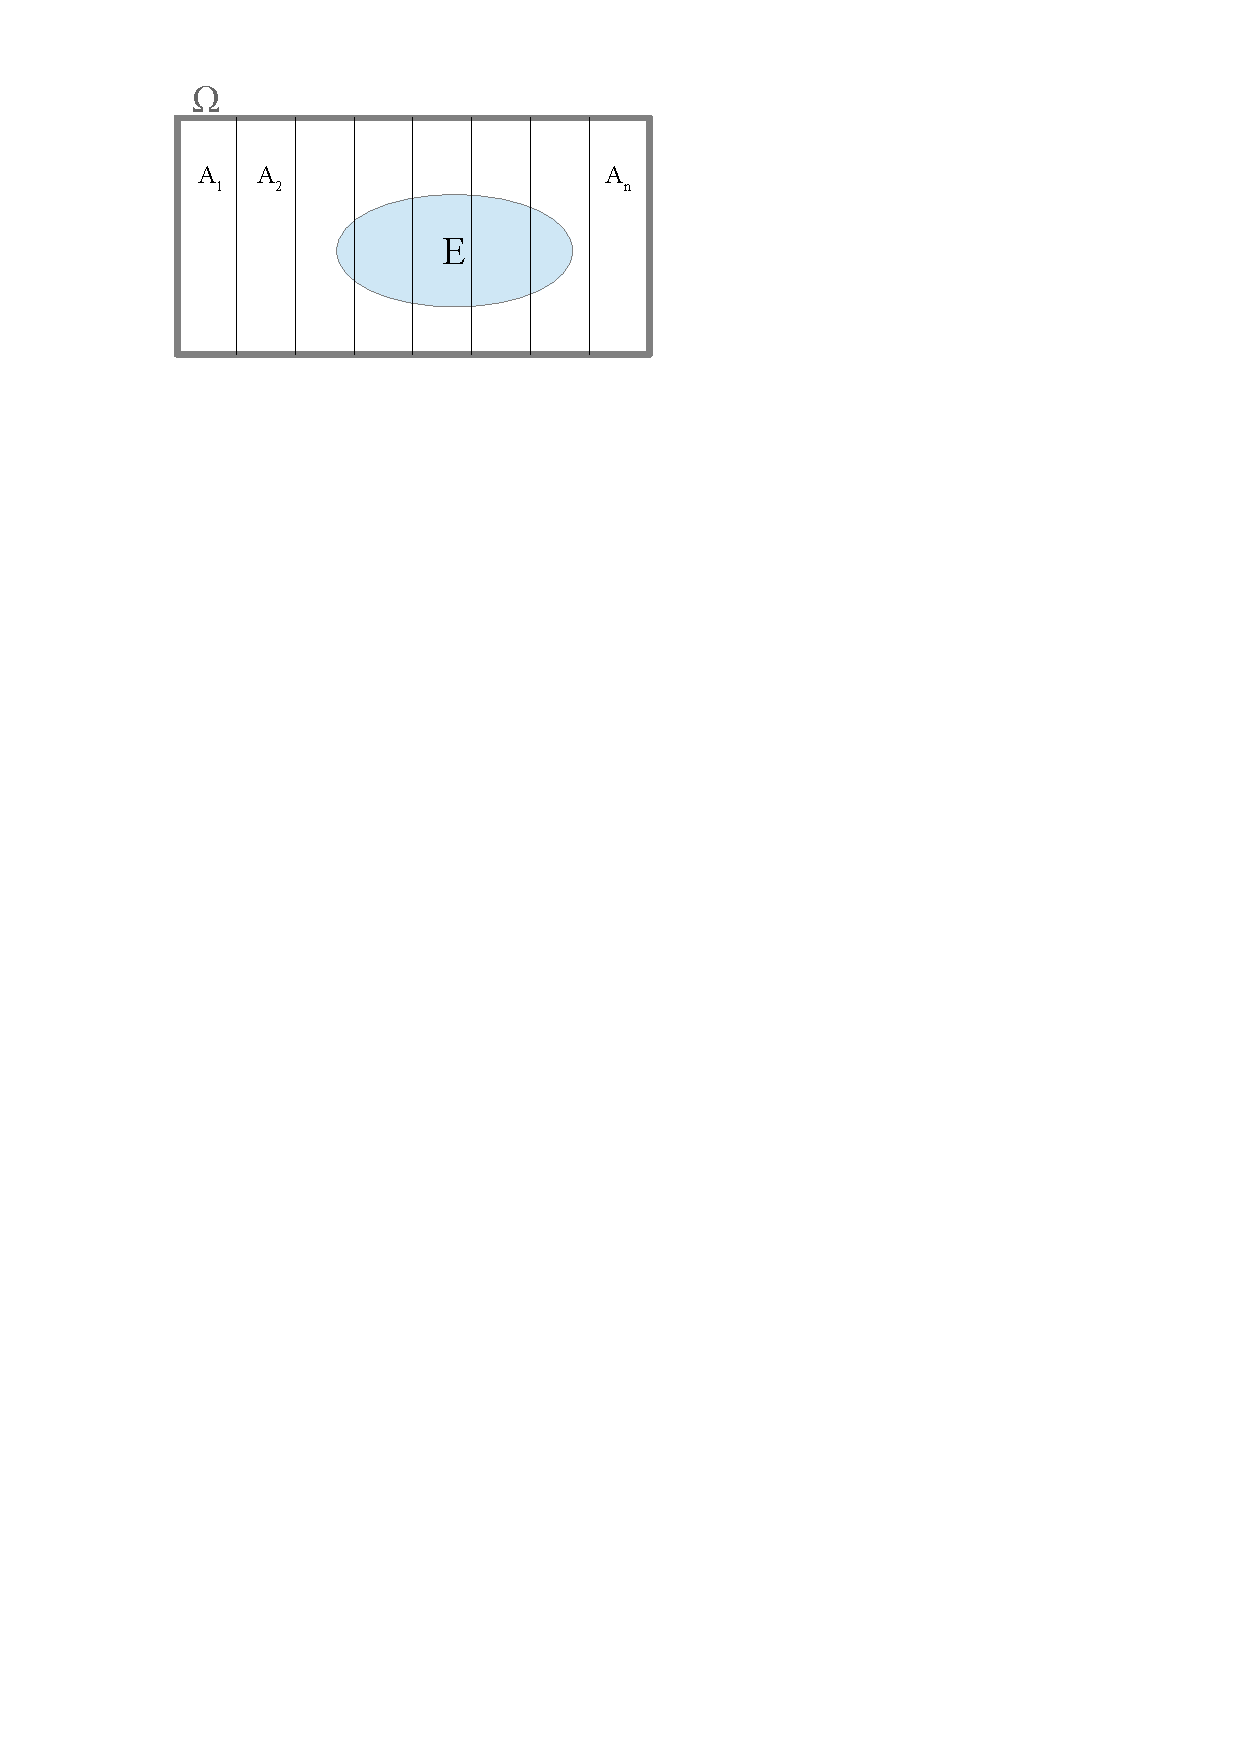
\includegraphics[width=5cm]{./Content/EreignisseWahrscheinlichkeit/total_probability.pdf}
  \end{minipage}
	
	\vspace{2mm}
	\hrule
	\vspace{3mm}
				
\subsection{Laplace event}
		In einem endlichen Wahrscheinlichkeitsraum $\Omega$ haben alle
		Elementarereignisse die gleiche Wahrscheinlichkeit.
		\begin{center}
		$P(A)=\dfrac{\left| A\right|}{\left|\Omega\right|}$
		\end{center}
		
	\vspace{2mm}
	\hrule
	\vspace{3mm}

\vfill
\newpage
	
	
